\chapter{Optimizations of NAS Algorithm}
\label{chap:nas_optimizations}

\begin{sloppypar}
While black-box Neural Architecture Search (NAS), as described in the Section~\ref{chap:nas}, offers a highly flexible and effective framework for discovering high-performing models, it is also notoriously resource-intensive and time-consuming. These limitations make it challenging to apply in real-world scenarios, particularly on constrained hardware as many discovered models will not be compatible to some microcontrollers. 
In this chapter, we present a set of optimization strategies aimed at enhancing the efficiency of black-box neural architecture search (NAS), with a particular focus on accelerating model evaluations and reducing overall search time—while maintaining the quality of the resulting architectures.
\end{sloppypar}

\section{Memory Estimation}

As previously discussed, one of the most significant challenges in this work was designing neural network architectures that fit within the strict memory constraints of the Arduino deployment environment. Initially, the process involved generating an architecture, training it, and attempting deployment—only to discover that the model exceeded the hardware limitations. 

This trial-and-error approach proved inefficient and was quickly abandoned. To address this, we developed a memory estimation mechanism capable of predicting the resource consumption of a model based solely on its architectural configuration. This allowed us to pre-screen candidate models and discard those unlikely to meet the deployment constraints, thereby accelerating the NAS process and conserving computational resources.

In addition, based on these memory estimations, we were able to predict secondary metrics such as inference time and energy consumption—values that previously required the model to be deployed in order to be measured. This advancement further streamlined the design and evaluation process.


To successfully deploy our neural network on the Arduino Nano 33 BLE Sense, we must account for the device’s limited usable memory resources—approximately 256KB of RAM and 1MB of Flash, though a portion of this is reserved for system operations, runtime overhead, and supporting libraries. As a result, the effective memory available for model deployment is lower than the hardware maximum. Any model that exceeds these practical limits is considered undeployable, regardless of its theoretical accuracy or performance.

While the most accurate way to measure memory usage is by compiling and deploying each model onto the microcontroller to observe its actual runtime behavior, this process is highly time-consuming and significantly reduces the number of models that can be evaluated within a given time frame. This is particularly, impractical when evaluating thousands of candidate architectures during Neural Architecture Search (NAS). Consequently, there is a critical need for fast and reliable approximation methods capable of predicting RAM and Flash consumption without requiring actual deployment.


Based on prior research \cite{tensorflow_RamEstimation}, \cite{liberis2019neural} , we make reasonable assumptions to model
memory consumption:

• RAM usage is estimated by analyzing activation tensor sizes during inference, considering their lifetimes and potential coexistence.

• Flash usage is initially approximated from the number of model parameters, then
corrected using a regression model to account for format overheads like quantization
metadata and FlatBuffer structure.

These assumptions allow us to perform fast memory estimations with reasonable accuracy, enabling effective filtering and prioritization of architectures before committing to
the costly deployment step. To improve the quality of these estimates, empirical data
was collected and regression models were trained to correct for systematic biases in the naive estimators. The resulting tools are embedded in the module, ensuring that only
deployable models are selected for further optimization

To fully understand the capabilities and resource limitations of our device, we conducted experimental analysis to identify the sources of memory overhead. This overhead arises from several essential components required for model execution and embedded functionality:

\begin{itemize}
    \item \textbf{Flash Memory Overhead:} In addition to the model weights and logic—stored in a \texttt{.h} file converted from a \texttt{.tflite} model and consuming the majority of board's memory, additional consumption arises from:
    \begin{itemize}
    
        \item \textbf{CMSIS-NN / Inference Functions:} Optimized functions responsible for executing the neural network layers (e.g., \texttt{arm\_nn\_softmax\_common}, \texttt{arm\_depthwise\_conv\_opt}, etc.) are stored in Flash memory. The more complex the model (i.e., more layers or operations), the more Flash these functions consume.
        
        \item \textbf{Arduino Sketch Code:} To deploy the model on the board, a sketch is used that includes constant variables, initialized pointers, additional libraries, static variables, and runtime logic. 

        \item \textbf{Embedded Input Data:} Input data used for testing (e.g., sample images) is stored as \texttt{const} arrays in Flash. While this contributes to Flash consumption, it avoids any additional RAM usage beyond the input tensor buffer already managed by the inference engine.

    \end{itemize}
\end{itemize}

\bigskip

\begin{itemize}
    \item \textbf{RAM Overhead:} Beyond the Tensor Arena—which is allocated specifically for intermediate buffers during inference—several other components consume RAM:
    \begin{itemize}
        \item \textbf{Main Stack} (\textasciitilde32~KB): Reserved for function calls, local variables, and handling interrupts. This ensures safe execution across diverse runtime scenarios.
        \item \textbf{Standard Library Buffers:}
        \begin{itemize}
            \item \texttt{impure\_data} (\textasciitilde2~KB) and \texttt{\_\_malloc\_av\_} (\textasciitilde41~KB): Internal allocations used by the newlib C library for dynamic memory and standard I/O handling.
        \end{itemize}
        \item \textbf{System Threads and OS Buffers:}
        \begin{itemize}
            \item \texttt{os\_timer\_thread\_stack}: Allocated for RTOS timer handling and related system threads.
        \end{itemize}
        \item \textbf{Peripheral and Communication Buffers:}
        \begin{itemize}
            \item Buffers used by \texttt{\_SerialUSB}, I2C interfaces (\texttt{Wire}, \texttt{Wire1}), and other hardware drivers consume variable RAM depending on their initialization.
        \end{itemize}
        \item \textbf{Static Objects and Runtime Metadata:}
        \begin{itemize}
            \item Instances like \texttt{\_ZZ5setupE8resolver} and static variables declared in the sketch occupy RAM during execution.
        \end{itemize}
        \item \textbf{Interrupt Handlers and Background Tasks:} RAM is also consumed by interrupt service routines (e.g., for BLE events, sensor data polling) and background OS tasks.
    \end{itemize}
\end{itemize}


Empirical measurements during deployment revealed that, in addition to the model's footprint, the following are typical overheads:

\begin{itemize}

    \item \textbf{Flash Usage:} Approximately 200--210~KB, depending on model complexity, the size of embedded data (e.g., input arrays), and the libraries included in the compiled sketch.
    
    \item \textbf{RAM Overhead:} Approximately 45--50~KB is consumed by system components, including the main stack, standard library buffers, RTOS threads, communication drivers, and runtime metadata. The remaining RAM is available for the Tensor Arena used by TensorFlow Lite Micro.

\end{itemize}








\subsection{Flash Memory Estimation}
\label{subsec:flash_memory_estimation}
Estimating the amount of flash memory needed to deploy a neural network model on a microcontroller is a crucial step in the development of edge computing applications, especially in environments where resources such as memory and processing power are severely limited. Flash memory, typically used as read-only memory (ROM), must store the model's parameters, which include the weights and biases of the neural network. These parameters define the behavior of the model and are essential for its operation during inference. A widely used method to estimate the flash memory requirement is to calculate the total storage needed for all the model's parameters. This involves summing up the memory footprint of each weight and bias, which are usually represented as floating-point or fixed-point numbers. By understanding the total number of parameters and their respective data types, developers can make an informed estimate of the memory space required for storing the model on a microcontroller. \cite{pau2023tiny}.

This method is fast and easy to compute, but it doesn't accurately reflect the size of a fully converted \texttt{.tflite} model due to additional overhead such as:
\begin{itemize}
    \item Quantization calibration parameters
    \item Padding and alignment used in FlatBuffer format \cite{manor2022custom}
\end{itemize}



The initial estimation function used the following logic:
\[
\text{Estimated Flash (KB)} = \frac{\text{Total Parameters} \times \text{Data Type Size (Bytes)}}{1024}
\]

This approach uses the \texttt{count\_params()} method from Keras and assumes a constant multiplier depending on data type. In our case, we have quantized the model, our datatype is int8 (1 byte).

While efficient, this method consistently underestimates the actual TFLite model size, which might allow bigger than the allowed to be trained while it will not fit in the deployment enviroment making it time consuming training something too big.

To verify accuracy, a dataset of real models was collected. Each model was:
\begin{enumerate}
    \item Built using Keras
    \item Converted to TFLite with full integer quantization
    \item Measured for actual file size in kilobytes
\end{enumerate}

The results showed a consistent gap between the estimated and actual sizes, motivating the use of a correction model.

We applied a simple linear regression model to learn the relationship between the estimated flash (param-based) and the actual flash (TFLite file size):

\[
\text{Corrected Flash Estimate} = a \cdot \text{Estimated Flash} + b
\]

Using a dataset of paired values, we trained the regression model and obtained the following parameters:
\[
\text{TFLite Size} \approx 1.1577 \cdot \text{Estimate} + 66.10
\]

 This model was saved using \textbf{joblib} and can be reused to instantly predict corrected flash estimates without invoking the TFLite converter.

 \begin{figure}[ht]
  \centering
  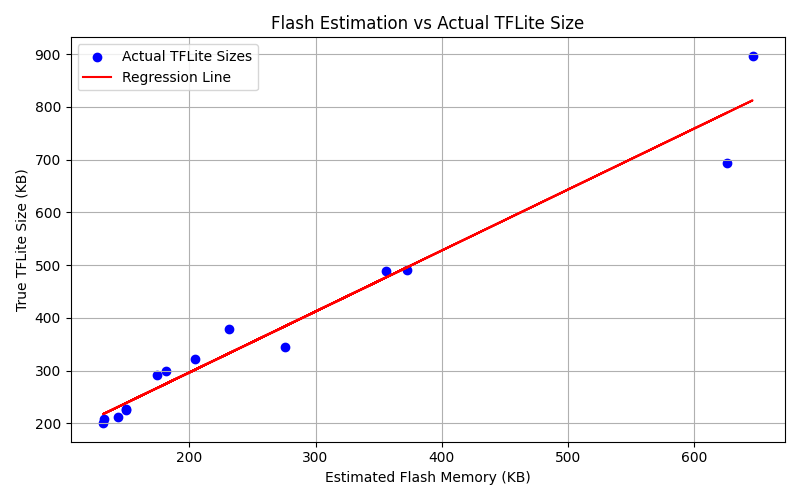
\includegraphics[width=0.85\textwidth]{Pictures/flash_regression_plot.png}
  \caption{Linear regression fit between estimated and true TFLite flash sizes.}
  \label{fig:flash-regression}
\end{figure}


Although the sample-based estimation is generally close to the actual deployment behavior, in cases where a model approaches the Flash memory limits, it is advisable to perform an early conversion to the \texttt{.tflite} format. This allows verification that the model fits within the memory constraints before proceeding with full training. The workflow consists of first converting the untrained Keras model to a TFLite version to ensure feasibility, then continuing with the regular training of the original Keras model, followed by conversion and deployment as usual.

Although this process introduces a small time overhead—typically just a few seconds—it is negligible compared to the cost of fully training a model, which can take around 20 minutes, only to later discover it cannot be deployed due to memory constraints. Conducting an early Flash feasibility check thus serves as a valuable safeguard, helping to avoid unnecessary training and conserve computational resources..

\clearpage

\subsection{Ram Memory Estimation}

During inference, each layer produces intermediate activation tensors that occupy RAM. However, not all intermediate tensors exist in memory at once – their lifetimes are limited to when they are being computed and used. A naïve approach (not reusing any buffer) would allocate a separate buffer for every intermediate tensor but this can lead to a huge memory footprint. \cite{tensorflow_RamEstimation} 


The key insight is that we can estimate the peak RAM usage by analyzing the sizes of activation tensors and understanding which ones coexist at runtime. Typically, the peak memory occurs at a layer where the largest combination of activations must be stored simultaneously. For sequential models (simple chains), this often boils down to the input and output of a single layer – once a layer’s output is produced, the previous activations can be released. \cite{liberis2019neural}

 A simplified but effective heuristic is to assume that the input and output tensors of each layer represent the concurrent memory needed during the computation of that layer, and take the maximum over all layers \cite{tensorflow_RamEstimation}. 

However, layers such as Concatenate introduce memory persistence, requiring previous activations to remain allocated until the merge operation completes. This forces multiple tensors to coexist in memory simultaneously, leading to overlapping memory demands. As a result, the real peak RAM usage can substantially exceed the simple input-output memory estimation.




As illustrated in Figure~\ref{fig:TakuNet}, our model architecture is organized into three main stages:

\begin{itemize}
    \item \textbf{Stem Block}
    \item \textbf{TakuStages Block}
    \item \textbf{Refiner Block}
\end{itemize}

The \textbf{Stem Block} and \textbf{Refiner Block} consist of consecutive layers without any additions or skip connections. Consequently, estimating the peak RAM usage for these blocks is straightforward—it corresponds to the maximum RAM required by any single layer within the block.

In contrast, each \textbf{TakuStage} includes residual operations, which require special consideration in memory estimation. Specifically, when performing concatenation or skip-connection, all input tensors must be available in memory at the same time to compute the output. This increases the peak memory footprint compared to purely sequential operations. To accurately account for this, we compute the peak RAM usage for each \textit{TakuStage} by identifying the maximum cumulative memory required across all active feature maps at any point in time. Let \( A_i \) denote the activation size of layer \( i \), and let \( \text{Live}(t) \) represent the set of layers whose outputs must remain in memory at time step \( t \). Then, the maximum RAM usage is given by:

\[
\text{MaxRAM} = \max_{t} \left( \sum_{i \in \text{Live}(t)} A_i \right)
\]

where
\[
\text{Live}(t) = \left\{ i \mid \text{output of layer } i \text{ is still needed for a future operation at time } t \right\}
\]

This formulation ensures that memory is only released after all dependencies have consumed the relevant activations.


To estimate the total maximum RAM required by the entire model, we take the maximum RAM usage from each of the three blocks and select the largest among them:

\begin{equation}
\text{RAM}_{\text{max}} = \max\left( \text{RAM}_{\text{Stem}},\ \text{RAM}_{\text{TakuStages}},\ \text{RAM}_{\text{Refiner}} \right)
\label{eq:max_ram}
\end{equation}

While the RAM estimation aligns closely with the actual measured RAM, it still tends to underestimate total memory usage due to the aforementioned memory persistence effects.

To better capture this discrepancy, we applied a similar approach as in  Section~\ref{subsec:flash_memory_estimation}, creating a linear regression model between the Estimated and Measured RAM values. The resulting line—referred to as \textit{LinearRAM}—reveals a consistent pattern in the mismatch, suggesting that a correction factor can be reliably modeled.

\begin{figure}[ht]
  \centering
  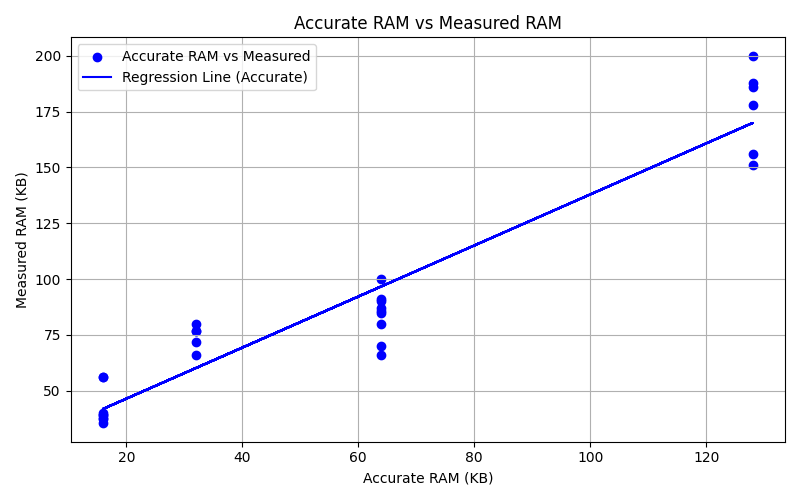
\includegraphics[width=0.85\textwidth]{Pictures/ram_accurate_vs_measured.png}
  \caption{Linear regression fit between estimated and true RAM consumption.}
  \label{fig:ram-linear-regression}
\end{figure}

\subsection{Energy Consumption Estimation}

Energy estimation is one of the most important aspects when deploying neural networks on microcontrollers, especially in power-constrained environments. The total energy consumed during a single inference can be expressed as:

\[
E = V \cdot \sum_{t=0}^{t_m} I(t) \cdot \Delta t
\]

where \( E \) is the energy in joules, \( V \) is the supply voltage (assumed constant), \( I(t) \) is the instantaneous current at time \( t \), and \( t_m \) is the duration of the inference.

In this work, the supply voltage was fixed at 3.3\,V using the Power Profiler Kit II. Figure~\ref{fig:current_profile} shows the measured current profile during a sequence of inference operations on the Arduino Nano BLE 33 Sense.

\begin{figure}[H]
    \centering
    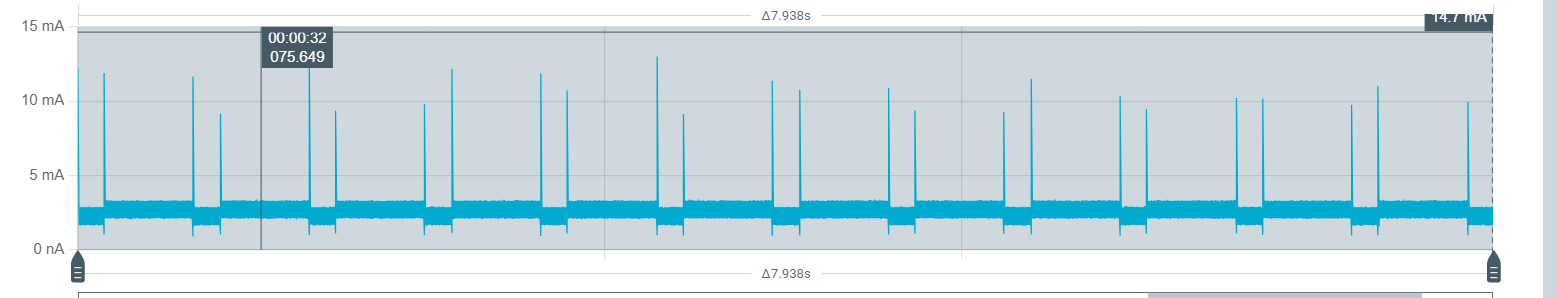
\includegraphics[width=\textwidth]{Pictures/Current.png}
    \caption{The current consumption observed during repeated model inference operations, with peaks corresponding to the active computation phases.}
    \label{fig:current_profile}
\end{figure}

As illustrated, the current remains relatively low during idle periods and exhibits distinct peaks during inference, where the processor becomes active. These peaks typically reach values around 10–15\,mA, while the baseline current hovers around 3–4\,mA.

This behavior reflects the nature of the microcontroller's operation: the Cortex-M4 CPU periodically wakes from low-power states to execute inference computations, then returns to idle. The CPU frequency—typically around 64\,MHz on the Arduino Nano BLE 33 Sense—determines how fast each instruction is executed. A higher frequency means that computations are completed faster, but it also implies more switching activity in the silicon, which increases instantaneous current draw.

However, our measurements show that the peak current is mostly determined by the processor architecture and workload type, and not by the specific neural network model. Consequently, the current profile \( I(t) \) remains relatively unchanged between models. The main variable that affects energy consumption is the inference time \( t_m \), which varies depending on the model's size and complexity.

Therefore, minimizing inference time directly contributes to energy savings, making it a key optimization objective in resource-constrained embedded AI applications.



\subsection{Inference Time Estimation}

Inference time refers to the duration a trained model requires to process an input and produce an output — essentially, the latency of a single forward-pass computation. In the context of embedded systems, inference time is a key metric, as it directly impacts both the responsiveness and energy consumption of a deployed model.

One important observation is that inference time is strongly influenced by the model’s memory (RAM) usage. 

On microcontrollers, where memory and computational bandwidth are both constrained, models that consume more RAM typically involve larger weight matrices or more extensive intermediate tensor storage. These factors increase the volume of memory access operations and place greater demand on the processor, resulting in longer inference durations.

Studies confirm that optimizing memory usage tends to speed up inference. For example, using fused in-place operations to reduce peak RAM footprint by about 1.6 × yielded a 1.2–2× faster inference execution in a TinyML context \cite{inferenceTime1}. Similarly, an embedded ML framework that lowered memory usage by 31\% achieved a remarkable 92\% reduction in inference latency compared to a less memory-efficient baseline~\cite{inferenceTime1}.


Those assumptions were confirmed after our test, finding a Linear corelation between the actual Measured RAM of the model and the inference time needed to produce the result.

\begin{figure}[ht]
  \centering
  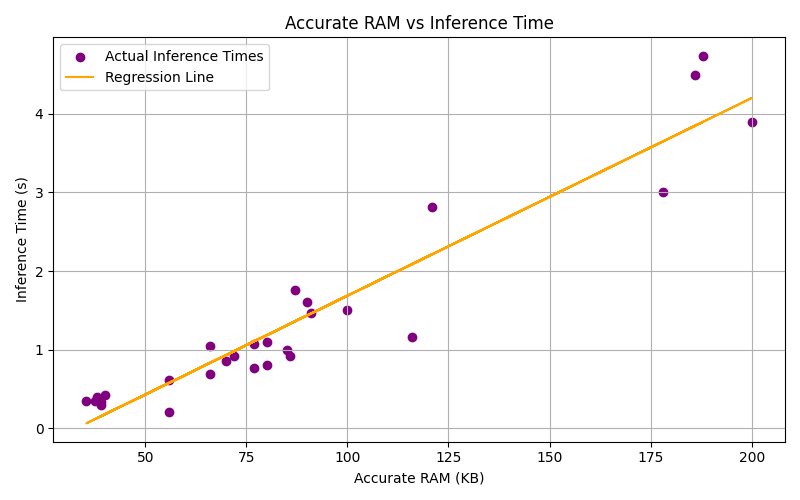
\includegraphics[width=0.85\textwidth]{Pictures/inference_time_regression_plot.png}
  \caption{Linear Corelation between RAM and Ιnference time.}
  \label{fig:inference time}
\end{figure}





\section{Model Comparison}
After the creation of the models in each new generation in the GA, we face the challenge on how to correctly choose the best models as parents for the upcoming generations and how to accelerate this procedure. So in the section the Tournament Selection and RankNet will be explained on how they tackle those issues. 

\subsection{Tournament Selection}
Tournament Selection (TS) is a genetic operator in which a small subset of individuals is chosen at random and the fittest among them is selected as a parent \cite{hussain2020trade}. 
Concretely, one chooses a tournament size \textit{k} and repeatedly samples \textit{k} individuals from the population. The individual with the highest fitness in each sampled group is declared the winner and used for reproduction \cite{hussain2020trade}.

Tournament selection inherently preserves population diversity and thus supports generalization. Because selection is based on competition within small random samples, occasionally sub-optimal individuals can win and propagate their genes \cite{hussain2020trade}.

In effect, TS avoids the extreme elitism of always picking the single best, which can lead to premature convergence. A well-designed selection should maintain diversity to avoid getting stuck in local optima \cite{filipovic2003fine}.

By keeping a variety of architectures in the gene pool, TS enables the GA to explore multiple promising regions of the search space. This broader search helps prevent overfitting to any one metric and tends to produce more robust CNN designs.





\subsection{RankNet}

In our initial approach, we trained all candidate models and then applied tournament selection (TS) to compare their performance. The top-performing models were subsequently selected to form the next generation. Through experimentation, we found that fully training each model before applying tournament selection was highly time-consuming, especially when many models were ultimately discarded. To address this inefficiency, we introduced \textit{RankNet}, a predictive model designed to estimate the relative performance of candidates without requiring any training.

\textbf{RankNet} is a pairwise ranking model originally developed for learning-to-rank tasks (e.g. search result ranking). It uses a shared neural network to map each input (here, an architecture embedding) to a score, then models the probability that one item is better than another by a sigmoid on the score difference \cite{RankNet}.

A key enabler for RankNet in NAS is a fixed-length embedding of each architecture that captures its structure. Recent works use graph-based embeddings; for example, Graph2Vec treats a neural network’s computational DAG as a “document” of rooted subgraphs (analogous to words) and learns a vector representation such that architectures with similar subgraph patterns are mapped close together in embedding space \cite{RankNet}.

Unlike graph-based embeddings (e.g., Graph2Vec), we use a handcrafted, lightweight embedding derived from the NAS search space parameters. Each architecture is represented as a fixed-size vector containing:
\begin{itemize}
    \item Normalized hyperparameters (e.g., filter counts, kernel sizes, strides) from all the blocks of the architecutre.
    \item One-hot encoded optimizer choices (SGD or AdamW),to be able to estimate even which optimized might fit better to the dataset.
\end{itemize}

This approach is computationally efficient and aligns with our fixed architecture template.

Once the models are embedded, a RankNet model is trained on a set of fully evaluated networks. Rather than regressing absolute accuracy values, RankNet learns to predict *relative* performance: given a pair of architecture embeddings, it estimates the probability that one outperforms the other. The model itself uses a shared 3-layer MLP (64 $\rightarrow$ 32 $\rightarrow$ 16 units) to process each architecture embedding. A sigmoid output predicts the probability that one model outperforms another, given their embedding difference:
\begin{equation}
    P(x_i \succ x_j) = \sigma(f(x_i) - f(x_j)),
\end{equation}

where $f(x)$ is the shared MLP's score for embedding $x$. Training uses binary cross-entropy loss on pairs of fully evaluated models.This strategy is advantageous because modeling relative fitness is often more robust
and data efficient than predicting absolute scores.


To avoid computational overhead and ensure fair comparison across runs, we train RankNet only once using the fully evaluated models from the \textbf{initial population}. This snapshot provides diverse training signals while ensuring consistency.

\begin{enumerate}
    \item \textbf{One-Time Training:} RankNet is trained only once at the beginning of the search process. This decision is primarily driven by efficiency: repeated retraining would introduce significant computational overhead. By limiting training to a single round on the initial population, we reduce runtime while still providing useful ranking guidance.

    \item \textbf{Active Correction:} During tournament selection, if RankNet favors an untrained model over a trained one, we train the untrained model and compare their true performance. If RankNet’s prediction was incorrect, we retain the better-performing model and use the misprediction as a penalty signal for RankNet—effectively updating its training data to reflect this mistake in the next retraining cycle.
\end{enumerate}

Although RankNet requires pairwise comparisons to learn, it does not demand a large number of individual models. Even with a relatively small initial population (e.g., 6-10 models), we can generate a quadratic number of pairs (up to $O(n^2)$), greatly expanding the effective size of our training dataset. In our implementation, we construct \textbf{all possible pairs} from the initial population. This step is computationally cheap and does not introduce any noticeable latency in the training pipeline.

\paragraph{Pair Generation Algorithm :}
Let $x$ be the number of fully evaluated models in the initial population. The total number of unique unordered model pairs that can be generated is:

\[
\text{Number of Pairs} = \binom{x}{2} = \frac{x(x - 1)}{2}
\]

This approach enables RankNet to learn from a rich set of comparisons, even when the initial number of fully trained models is relatively small. By generating all possible pairs, we achieve data-efficient training without introducing computational overhead. In doing so, our design strikes a careful balance between efficiency and generalization: RankNet helps avoid the costly full training of weak candidates during selection, while preserving fair, one-time evaluation behavior that aligns with real-world deployment constraints.


\begin{comment}
    However, during the early stages of evolution, the RankNet model is not yet reliable due
to limited training data. To address this, we adopt two key strategies:
\begin{enumerate}
    \item \textbf{Progressive Refinement:} As the search progresses, we accumulate an increasing number of fully trained models. After each generation, we retrain the RankNet using the new pairwise comparisons, allowing the model to incrementally improve its ranking accuracy.
    
    \item \textbf{Active Correction:} During tournament selection, if RankNet favors an untrained model over a trained one, we train the untrained model and compare their true performance. If RankNet’s prediction was incorrect, we retain the better-performing model and use the misprediction as a penalty signal for RankNet—effectively updating its training data to reflect this mistake in the next retraining cycle.
\end{enumerate}

These mechanisms help RankNet adapt over time and increase the reliability of its predictions, ultimately leading to a more efficient and informed neural architecture search.
\end{comment}






\section{Speed-Up in Training}

Once a model is selected—either as part of the initial population or through evolutionary selection—it must undergo full training to evaluate its true performance. Given the potentially large number of candidate architectures evaluated during the search, reducing training time becomes crucial for overall efficiency. Therefore, we implemented several optimization strategies to accelerate the training process, without significantly compromising the quality of the resulting models. These strategies aim to minimize unnecessary computational overhead, enabling faster feedback loops within the NAS cycle and more rapid convergence.

\subsection{Performance STOP}
\label{sec:performance_stop}
To reduce the training cost in Neural Architecture Search (NAS), we introduce two early stopping criteria based on the validation performance trajectory of candidate architectures. These rules help terminate unpromising models before exhausting the full training budget.

Let \( A(t) \) denote the validation accuracy at epoch \( t \), and let \( T \) be the total number of epochs.

We define two criteria:
\begin{itemize}


 \item \textbf{Diminishing-returns rule}: Training is stopped if, within a continuous window of length \( \alpha T \) epochs (where \( \alpha \in (0,1) \)), the relative improvement in validation accuracy is less than a threshold \( \epsilon \). Formally, define a window \( [t, t+\alpha T] \), and stop training if:
  \[
  \frac{A(t+\alpha T) - A(t)}{A(t)} < \epsilon
  \]
  This rule captures cases of strongly diminishing returns, where continued training yields minimal gains. If the model has not shown meaningful progress during this window, it is reasonable to assume that the remaining training budget will have limited impact.

   \item \textbf{No-improvement rule}: Training is halted if the validation accuracy does not improve for a fixed number of consecutive epochs, denoted \( \tau \). That is, for \( \tau \) epochs:
  \[
  A(t) \leq A(t-1) \leq \dots \leq A(t-\tau)
  \]
  This acts as a safeguard for detecting early stagnation, even before the diminishing-returns window is reached.

\end{itemize}


These complementary criteria allow for early termination of underperforming models based on either slow progress or complete stagnation. Empirical evaluations across various NAS runs with different training budgets (e.g., 30, 50, 70 epochs) revealed that this strategy consistently reduces training time without degrading the fidelity of model selection. Inspired by recent NAS literature that advocates for efficient search through performance-based early termination \cite{li2020random}, we incorporated both rules into our pipeline.

After extensive experimentation, we identified the following parameter configuration as the most effective trade-off between training efficiency and selection reliability:

\begin{itemize}
  \item \textbf{Patience} \( \tau = 4 \): Maximum number of epochs allowed without improvement.
  \item \textbf{Window size} \( \alpha = 0.25 \): Fraction of total epochs used for evaluating diminishing returns.
  \item \textbf{Minimum relative improvement} \( \epsilon = 0.05 \): Threshold below which training is stopped.
\end{itemize}

This configuration significantly reduces the average training time per model while maintaining a low misranking error and preserving the integrity of the NAS process.

\begin{comment}
In many cases, if the validation accuracy does not show meaningful improvement after a certain number of epochs, training can be safely stopped early. The rationale is that even with additional training, the model’s performance is unlikely to increase substantially, and therefore its overall fitness score will remain largely unchanged. This idea is supported by recent NAS studies that implement early termination strategies to speed up the search process without compromising model selection accuracy \cite{li2020random}. By terminating such models early, we avoid wasted computation while still preserving a reliable basis for comparison with other candidate architectures. This strategy helps reduce the total search time while maintaining the fairness and effectiveness of the NAS process.
\end{comment}








\begin{comment}
    


\subsection{Early Stopping}
\TODO{Read this to see if it is good enough}
Research indicates that during CNN training, the initial few epochs often yield the most significant gains in model learning, strongly shaping the network’s eventual accuracy. In other words, a large portion of a CNN’s final validation performance is determined early in training. The following are key findings from credible sources that support this idea.

In an analysis of “critical learning periods,” the authors found that “the first few epochs are critical for the creation of strong connections” in a neural network, after which these connections “do not appear to change during additional training.” They conclude that this initial learning phase “plays a key role in determining the outcome of the training process.” In practice, most of the network’s representational capacity and generalization ability is established in these early epochs \cite{achille2017critical}

In Figure~\ref{fig:val_accuracy}, the normalized validation accuracy of several \texttt{TakuNet} models is shown across training epochs. It is evident that for all four models, the biggest part of the final validation accuracy is reached within the first few epochs. Specifically, by epoch 5 out of 30—that is, just \( \frac{5}{30} \times 100 = 16.7\% \) of the total training time—each model already achieves $\sim 70\%$ of its eventual accuracy and by epoch 10 out of 30—that is, just \( \frac{10}{30} \times 100 = 33.4\% \)  of the total training time—each model already achieves $\sim 80\%$ of its eventual accuracy . This highlights the efficiency of early training and suggests that prolonged training may offer diminishing returns.

In order to speed up the entire NAS algorithm, a Custom Callback method was introduced, which measured the validation accuracy of the model at the most important epochs. If the validation accuracy did not exceed a specific threshold, the algorithm abandons the model as it is pointless to spend more training time to a non-optimal model based on its constraints.
\end{comment}



\subsection{Early Stopping}
\label{sec:early_stopping}

Extensive research has shown that the early stages of convolutional neural network (CNN) training contribute disproportionately to a model's eventual performance. In particular, the first few epochs are often decisive in shaping the network's representational capacity and generalization ability.

A notable study on “critical learning periods” reports that “the first few epochs are critical for the creation of strong connections,” which “do not appear to change during additional training” \cite{achille2017critical}. The authors conclude that this early phase plays a central role in determining the final outcome of training. Empirically, this suggests that much of a CNN’s final validation accuracy is achieved early in training, and that continued training yields diminishing returns.

Figure~\ref{fig:val_accuracy} illustrates this effect for several \texttt{TakuNet} models. The normalized validation accuracy curves reveal that:
\begin{itemize}
  \item By epoch 5 out of 30 (just \( \frac{5}{30} \times 100 = 16.7\% \) of the total training time), each model achieves approximately 70\% of its final validation accuracy.
  \item By epoch 10 (33.4\% of training), the models have already reached around 80\% of their eventual performance.
\end{itemize}

These observations highlight the efficiency of early training and support the use of early stopping mechanisms to reduce unnecessary computation.

To leverage this behavior in our NAS pipeline, we introduced a custom callback mechanism that monitors validation accuracy at a strategic checkpoint. If the accuracy fails to exceed a predefined threshold by a specific fraction of the training process, the model is deemed unpromising and discarded early. Formally, let \( A(t) \) denote the validation accuracy at epoch \( t \), and let \( T \) be the total number of training epochs. We define an early termination condition as:

\[
A(t) < A_{\min} \quad \text{where} \quad t = \lfloor \beta \rfloor
\]

Here, \( \beta \in (0,T) \) represents the early evaluation point, and \( A_{\min} \) is the minimum acceptable validation accuracy at that point.

After extensive experimentation across multiple runs and training durations, we found that this early stopping rule was effective in filtering out weak models without degrading overall NAS performance. It significantly accelerated the search process by terminating unpromising architectures early, thereby saving substantial computation while maintaining model selection quality.

Notably, we observed that the optimal values for the evaluation point \( \beta \) and the minimum acceptable accuracy \( A_{\min} \) vary depending on the total number of training epochs. However, for any fixed number of training epochs, these values remained stable and consistent across experiments. This indicates that early stopping parameters can be reliably tuned for each training schedule and reused without the need for frequent adjustment.



\begin{figure}[H]
    \centering
    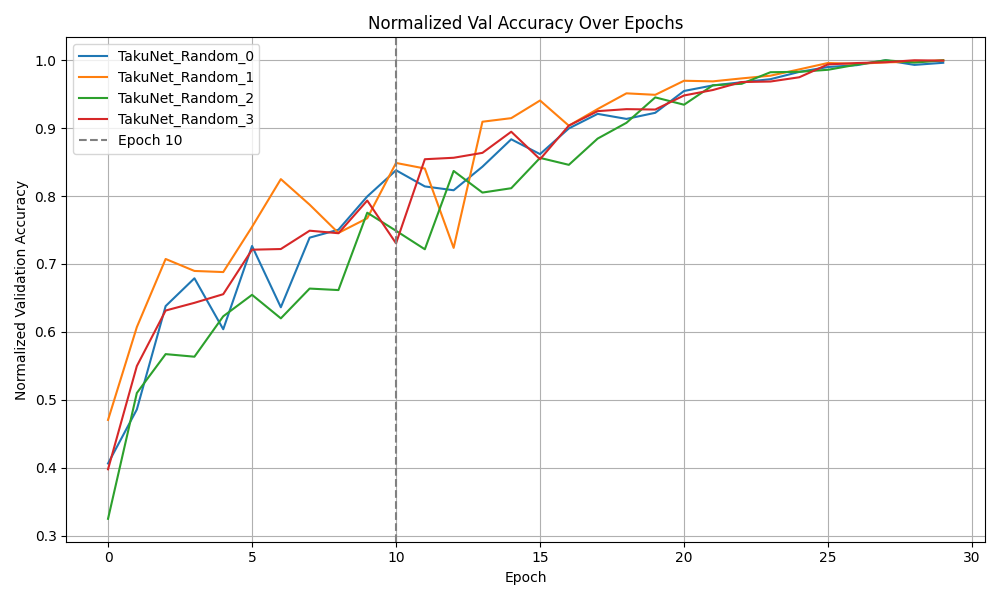
\includegraphics[width=0.85\linewidth]{Pictures/val_accuracy_comparison.png}
    \caption{Normalized validation accuracy curves for different TakuNet variants.}
    \label{fig:val_accuracy}
\end{figure}




\subsection{Learning Rate Scheduling}

To accelerate convergence and improve generalization, we employed a cosine annealing learning rate schedule with a linear warm-up phase of 5 epochs. This strategy adjusts the learning rate dynamically across training: starting from a small value, rising linearly during warm-up, and then decaying smoothly according to a cosine function relative to the total number of epochs. 

The cosine function used ,inspired by \cite{loshchilov2016sgdr} : 

\begin{equation}
\text{lr}(t) = \eta_0 \cdot \frac{1}{2} \left( 1 + \cos\left( \frac{\pi (t - T_\text{warmup})}{T_\text{total} - T_\text{warmup}} \right) \right),
\end{equation}

where:
\begin{itemize}
  \item \( \eta_0 \) is the initial learning rate,
  \item \( T_\text{warmup} \) is the number of warmup epochs,
  \item \( T_\text{total} \) is the total number of training epochs,
  \item \( t \) is the current epoch number.
\end{itemize}


Cosine learning rate schedules have been widely adopted in modern image classification models such as ResNet, DenseNet, and MobileNet, and are considered state-of-the-art for datasets like CIFAR-10 and CIFAR-100~\cite{lewkowycz2021decay}. Studies show that cosine decay leads to faster convergence and slightly improved final accuracy compared to traditional step-based schedules.

As illustrated in Figure~\ref{fig:val_accuracy_diff_epochs}, for a TakuNet model, increasing the number of training epochs does not significantly improve validation accuracy, given the Learning Rate Scheduling technique used. This saturation effect aligns with the theoretical behavior of cosine decay: once the learning rate approaches zero, further updates become minimal. Given that each epoch takes approximately one minute to complete, it is computationally efficient to limit training to around 10 epochs—achieving nearly optimal results in a fraction of the training time and is sufficient to be able to compare models.

As a result, experiments where conducted to find the sweet spot of reducing the number of epochs while retaining  as low as possible the correct prediction on which model is better than the other

\begin{figure}[ht]
    \centering
    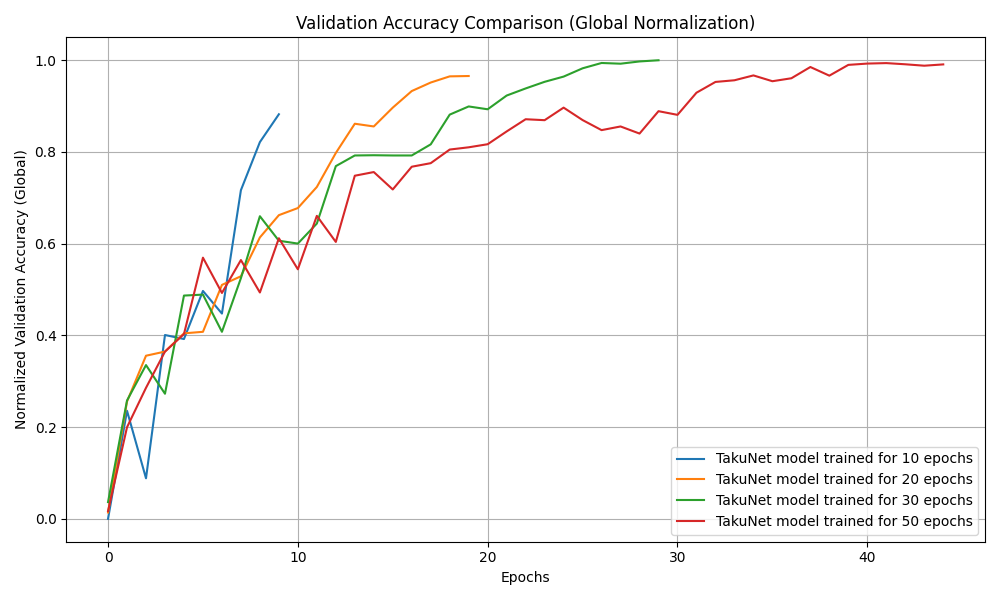
\includegraphics[width=0.85\linewidth]{Pictures/val_accuracy_comparison_global.png}
    \caption{Normalized Validation accuracy(based on highest recorder accuracy) of TakuNet trained for different number of epochs }
    \label{fig:val_accuracy_diff_epochs}
\end{figure}